\documentclass{article}
\usepackage{hyperref}
\hypersetup{colorlinks=true,urlcolor=blue}
\usepackage{listings}
\usepackage{geometry}
\geometry{margin=1in}
\usepackage{graphicx}
\graphicspath{ {./hw2/} }
\begin{document}
\title{BMI 203: Algorithms - Homework 2}
\author{Laurel Estes}
\maketitle
\section{Implementing Hierarchical and Parition-Based Clustering}
\subsection{Similarity Metric}
Given the limited scope of the project, I chose to implement a very basic (and to a large extent arbitrary) similarity metric, which is to calculate a linear combination of the following: length of the active site (in number of residues), surface area-to-volume ratio of the active site in space, and (given two sites for which similarity is being measured) the euclidean distance between the 6-element vectors formed by the percentages of residues in each site belonging to each of 6 physiochemical categories of amino acid (nonpolar, cysteine, polar uncharged, positive, negative, and bent). Active sites of enzymes rely on their physical shape and their local chemistry in order to catalyze reactions, and I wanted my metric to attempt to get at these properties without relying on amino acid sequence. My reasoning was that (for this project) I am most interested in trying to cluster sites that bind similar ligands, and for this purpose, the amino acid chemistry is more important than the amino acid identity, unlike in a DNA sequence. Furthermore, residues in sites are not necessarily a single continuous part of the protein, the residues are not necessarily arranged such that a linear sequence of residues maps well onto the structure for purposes of understanding local chemistry information. \par
Given more time, I would have liked to try to compare overall shape/size by overlaying the boxes formed by the active site dimensions, and potentially integrate some component of amino acid sequence data to try and capture information about what residues are next to each other (are there patches of polar vs nonpolar, etc.) I spent some time reading up on the PARIS algorithm (Hoffmann et al., 2010) and liked their general methodology of combining volumetric measurements with alignments of "probability clouds" of physical structure in order to try and cluster active sites based on similarity of the ligands that they bind. \par
Since we are given a fixed set of data, I made histograms of the similarities obsserved between every pair of sites in the set. I find it interesting that the combined metric (which I ended up using) has a very close to normal distribution centered around 0.51, while both of the two major components (which each contribute to 50\% of the similarity value) have very non-normal-looking distributions. I spent a brief amount of time qualitatively testing what happened when I used only one of the two major components (chemical similarity vs dimensional information) in isolation, with the idea that perhaps a non-normal distribution would be more likely to have inherent clusters rather than a uniform field of points (which a normal distribution seems like it might be suggesting...).
\begin{figure}[h]
\centering
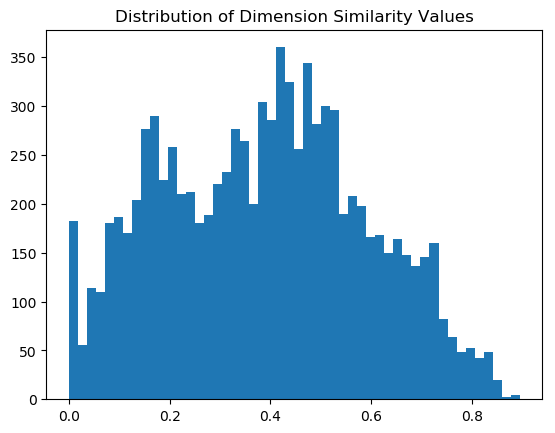
\includegraphics[width=0.31\textwidth]{./similarity_histogram_dim.png}
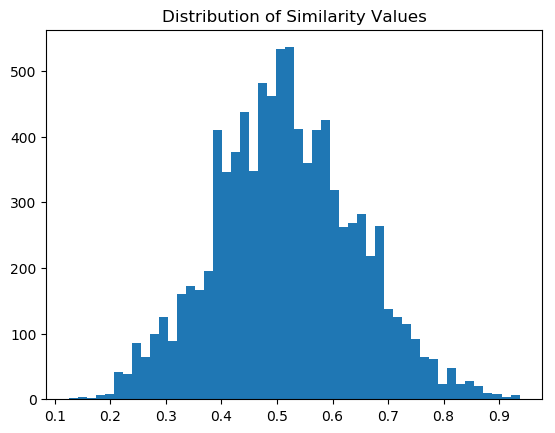
\includegraphics[width=0.31\textwidth]{./similarity_histogram.png}
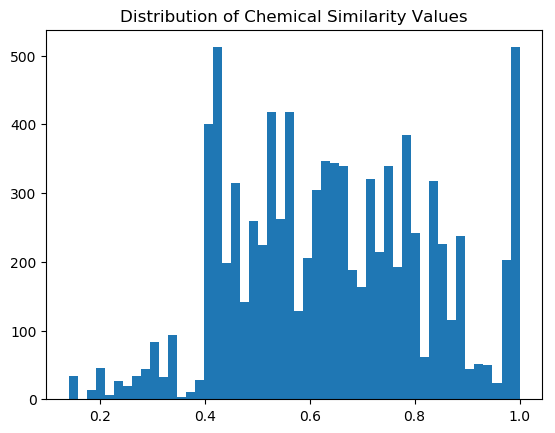
\includegraphics[width=0.31\textwidth]{./similarity_histogram_chem.png}
\end{figure}
\subsection{Hierarchical Algorithm}
For my hierarchical algorithm, I used an agglomerative (bottom-up) method with average-distance linkages, where I measured the similarity between centroids of the clusters (calculated by averaging the coordinates of each point in the cluster) and then calculated distance as a function of similarity as follows: $$\frac{1}{1-similarity}$$ 
I chose a nonlinear distance function partially just because I wanted to try it out and partially because I theorized that magnifying the similarities of closer sites would be more likely to create cluster-like structures (note that this is a terrible idea to do for real data unless you have a strong rationale as to why any cluster results produced would still be interesting and interpretable, not just pretty). After the distances between all the centroids of all the clusters were calculated, the two clusters with the shortest intervening distance were grouped into a single cluster, and the process is repeated until the input k number of clusters is achieved. In implementing this algorithm, I was concerned intially with having to recalculate the graph of inter-cluster distances every iteration, when only one new cluster is being made each time, so I created a Cluster class that stores its centroid coordinates, and also modify a single persisting graph representation of the clusters rather than re-creating it at each step. In retrospect, the Cluster class was superfluous, and caused some trouble when trying to avoid code duplication while writing the partitioning code without Cluster objects. Three examples (k=2,3,4) of clusters created by this algorithm are shown as colorations of the active sites projected into PCA space (see code and comments in graphing.py), and while we can see that the clusters do generally sort themselves along PC1, their "cluster-ness" quality by visual inspection is very dubious:
\begin{figure}[h]
\centering
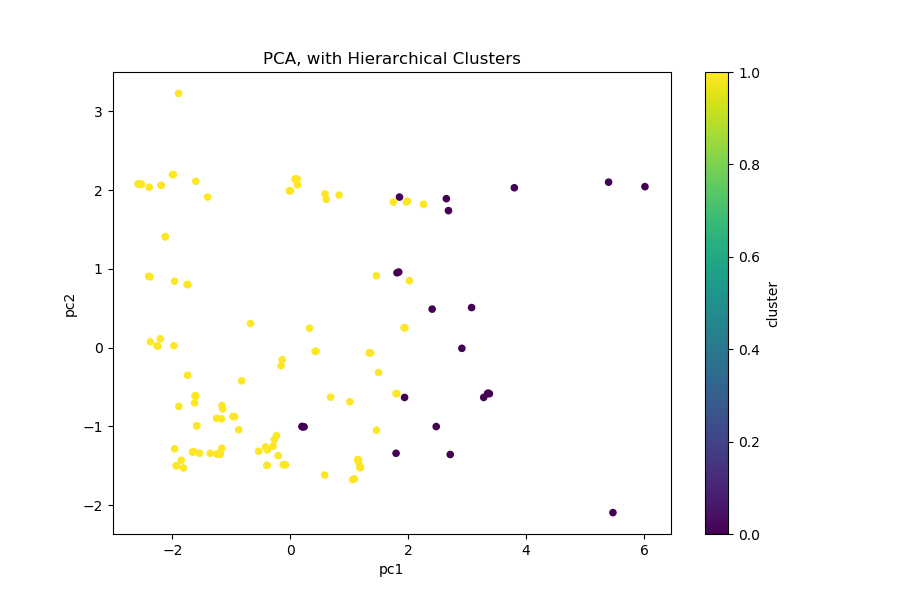
\includegraphics[width=0.45\textwidth]{./pca_h_k2.png}
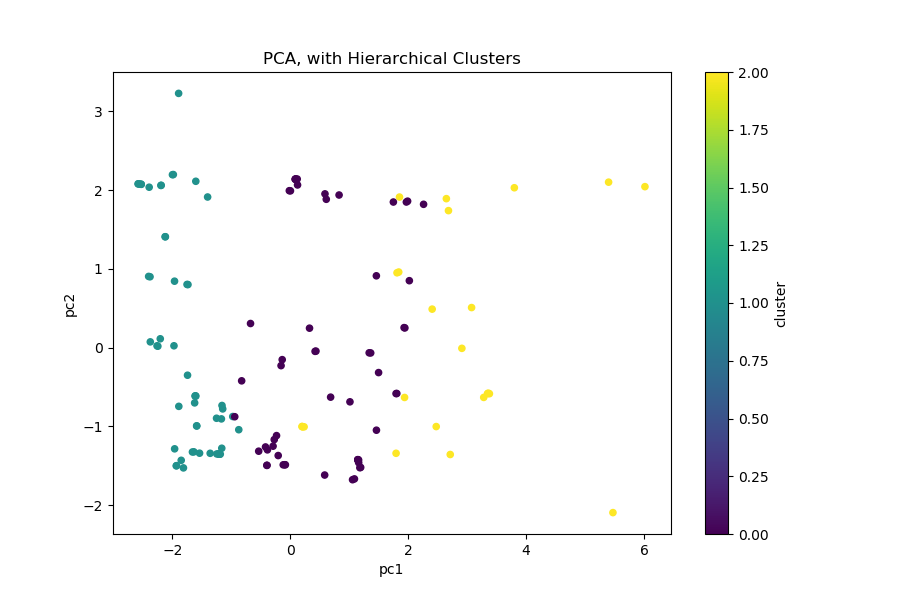
\includegraphics[width=0.45\textwidth]{./pca_h_k3.png}
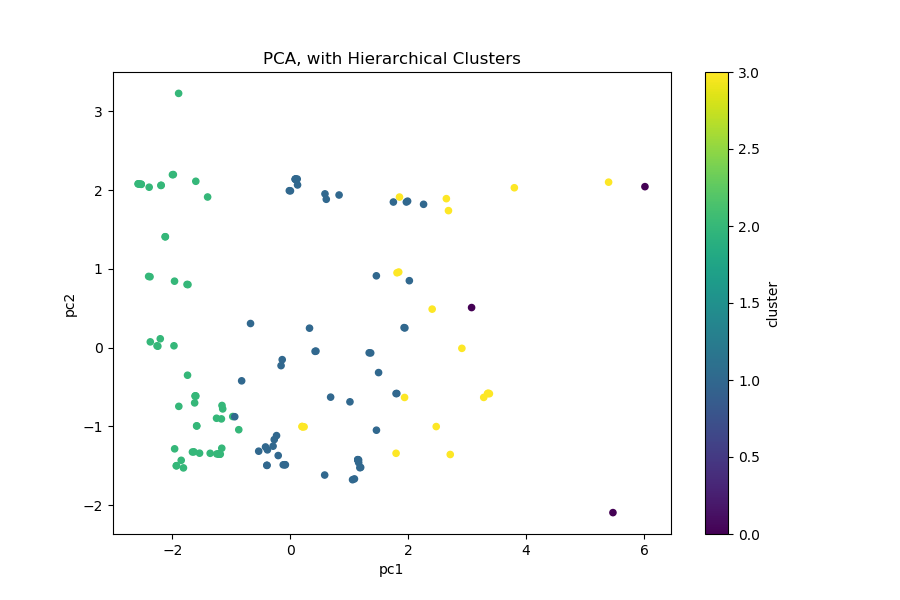
\includegraphics[width=0.45\textwidth]{./pca_h_k4.png}
\end{figure}
\subsection{Partioning Algorithm}
For my partitioning algorithm, I would have liked to try to implement CURE, which is a derivative of k-means that is better able to find non-spherical clusters, and clusters that vary more widely in relative size. It does this by contracting a set of multiple, distributed points within a cluster in each iteration instead of a calculating and repositioning a single centroid point. However, given time constraints, I implemented a very basic k-means algorithm instead. The k-means algorithm consists of two primary steps that are typically iterated until the change between iterations is below some threshold distance. First, k points (ideally far apart) are selected as the initial centroids of the k clusters. Second, all the remaining points are assigned to one of the k clusters based on which cluster's centroid is closest to that point. Then, the centroid positions are recalculated based on the coordinates of the cluster's new members, points are reassigned to the cluster with the closest centroid, and the process repeats. I ran into some issues in this algorithm with finding a good threshold distance for terminating the iterations; probably more dynamic programming than I had time to implement would have solved the problem more intelligently, but in this case, I made the iterations stop additionally if the exact same change-in-centroid-coordinates distance repeats, since that indicates a static jittering of the clusters between two states rather than an evolution towards any further optimization. Three examples (k=2,3,4) of clusters created by this algorithm are shown as colorations of the active sites projected into PCA space (see code and comments in graphing.py), and they are similar but not identical to the ones obtained by the hierarchical algorithm above. Notably, in k=3 and k=4, they start to segment along PC2 as well as PC1, instead of becoming thinner vertical clusters along PC1 as in the hierarchical method. Also, at k=4, these clusters qualitatively look much better than the hierarchical clusters at k=4 (one of the k=4 hierarchical clusters is just three, distant-in-PCA-space points), which may get to some underlying differences in the regimes of k at which each clustering method is at its best. (Alternately, given the not-very-clustered distribution of the data itself, this could be more of an underlying differnence in what noise/artifacts look like for each algorithm.)
\begin{figure}[h]
\centering
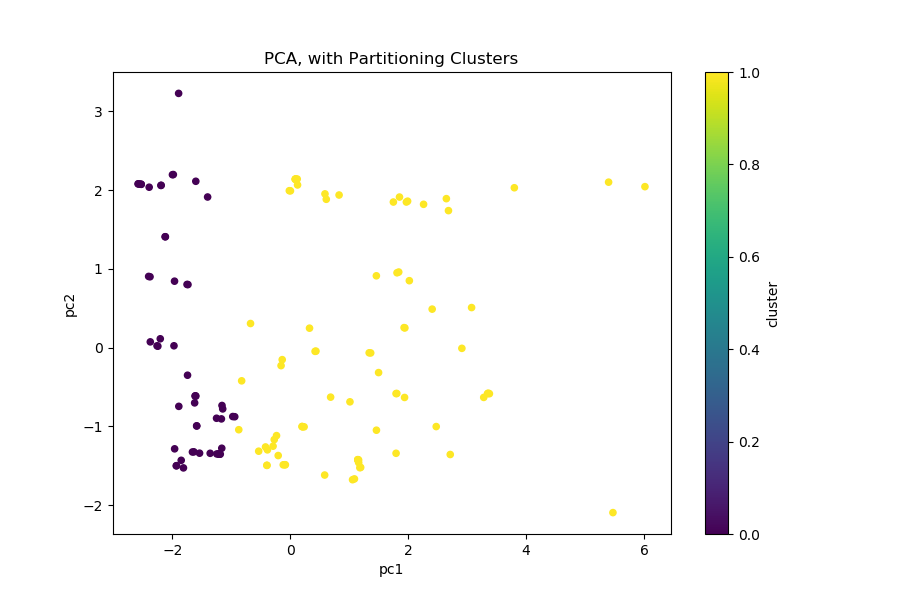
\includegraphics[width=0.45\textwidth]{./pca_p_k2.png}
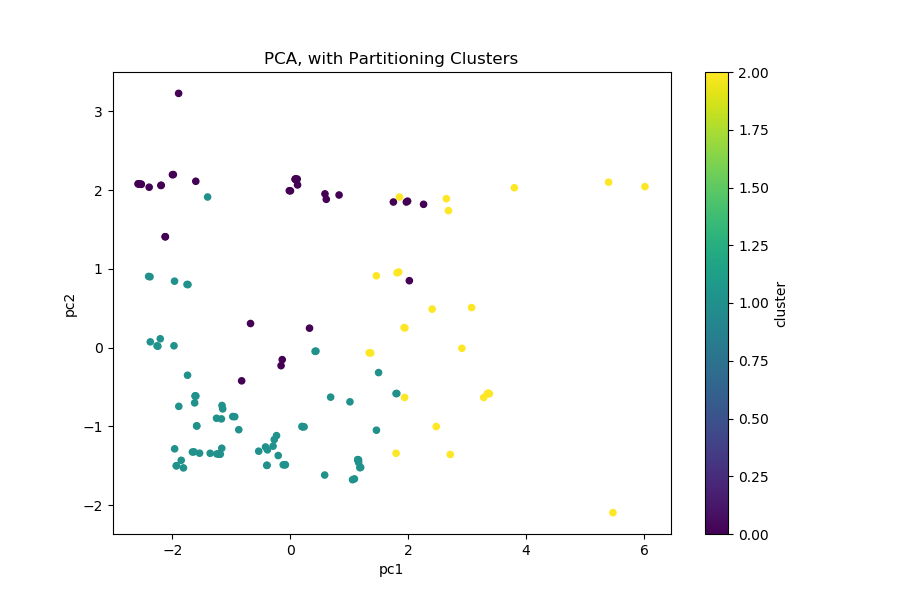
\includegraphics[width=0.45\textwidth]{./pca_p_k3.png}
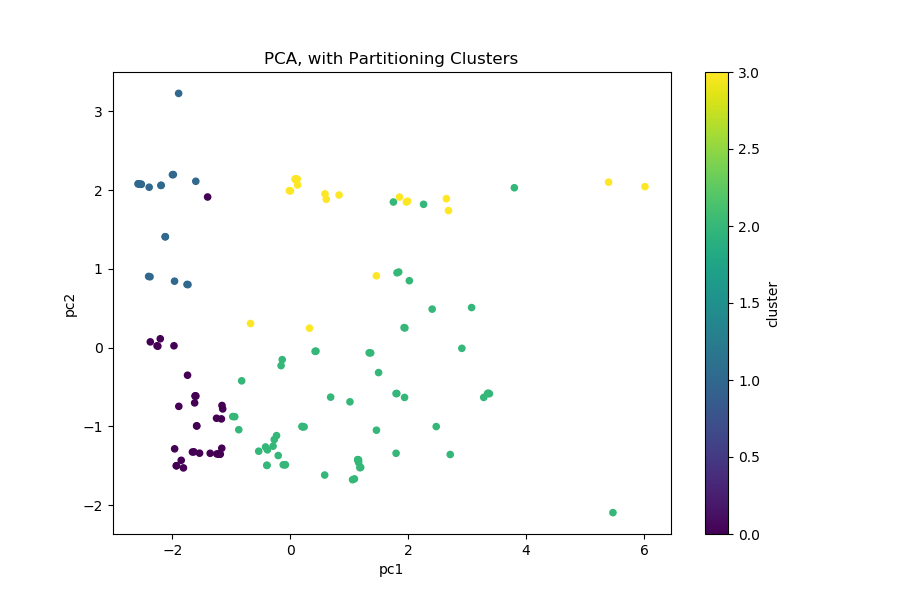
\includegraphics[width=0.45\textwidth]{./pca_p_k4.png}
\end{figure}
\subsection{Quality Measurement}
To measure cluster quality, the most straightforward metric I thought of was to compare intra-cluster similarity to inter-cluster similarity, for each cluster in a clustering. Good clusterings would have high intra-cluster similarity and low inter-cluster similarity, while clusters that were more similar to each other than internally would seem to be essentially spurious, since they do not contain a higher ``similarity density'' than their surroundings. Some more sophisticated statistics than simply taking the means and standard deviations across all points in a cluster and all clusters in a clustering would have been nice, but given time constraints, that was how I implemented this metric. Notably, despite its blunt-instrument averaging, this metric gives the intuitive result that NONE of the clusterings I was able to find, save one, had mean intra-cluster to inter-cluster ratios greater than 1--in other words, none of these clusters actually make sense as clusters. The one clustering I was able to create with a ratio greater than one was by using an altered similarity metric which just considered the chemical composition component, but the standard deviation was so high as to make the mean value essentially meaningless:
\begin{figure}[h]
\centering
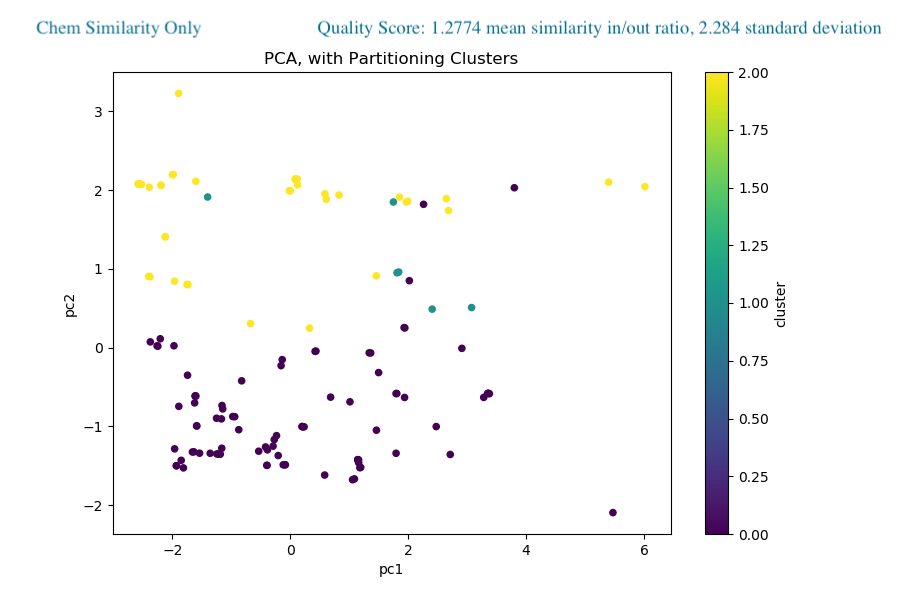
\includegraphics[width=0.45\textwidth]{./unicorn.png}
\end{figure}
\subsection{Comparing Clusterings}
To compare clusterings, I made a simple function that takes in two clusterings of the same length (e.g. equal k), displays the lengths of all the clusters in both clusterings, and calculates the counts of shared sites in each pair of clusters. This does not return a single aggregate value, although it could with some more work, but allows for a quick, general idea of how similar two clusterings are. Clusterings where the constituent clusters are very different lengths are obviously not very similar, and also, the more that the sites are spread out through all the combinatorial possibilities (e.g, some in clustering A cluster 1/clustering B cluster 2, some in A1/B5, some in A1/B1, etc.), the less similar the clusters are. This function is wrapped into the main function call of the module and writes to the output file when the '-C' (comparison) option is called instead of '-P' or '-H'.
\subsection{Biological Relevance}
Given the truly non-cluster-conducive nature of the variable space in which I chose to attempt to cluster, evinced by the uniformly more-similar-to-other-clusters-than-within-themselves nature of the clusters that both algorithms produced (from k=2 to k=8, with one test at k=65), I do not thing there is a strong biological relevance to these clusters. It seems like both of the major components of my similarity metrics are distributed more continuously than in clusters of values, within this data set. Additionally, the information sources I chose to try to use to cluster with may not be particularly biologically relevant, at least in the level of detail of their treatment here in my code. My choice of categories for the amino acids may not have been optimal (too many categories? No measure for overall size of the residue?); the overall shape of the active site is much more indirectly relevant to ligand binding than the interior geometry of the binding pocket; finally and probably the most impactful of all, the measures I chose are likely far outweighed in their importance to ligand binding by other, more difficult to compute factors, such as the exact sterics and local chemical environment of a few key residues in the binding pocket itself. 


\section{Github Repository}
All of the code used in this assignment is on Github: \url{https://github.com/laueste/algorithms-ucsf-2019}
\end{document}